%%%%%%%%%%%%%%%%%%%%%%%%%%%%%%%%%%%%%%%%%%%%%%%%%%%%%%%%%% 
\section{ハミルトン閉路問題とその関連問題}\label{chap:background}
%%%%%%%%%%%%%%%%%%%%%%%%%%%%%%%%%%%%%%%%%%%%%%%%%%%%%%%%%% 

%%%%%%%%%%%%%%%%%%%%%%%%%%%%%%%%%
\begin{figure}[tb]
  \centering
  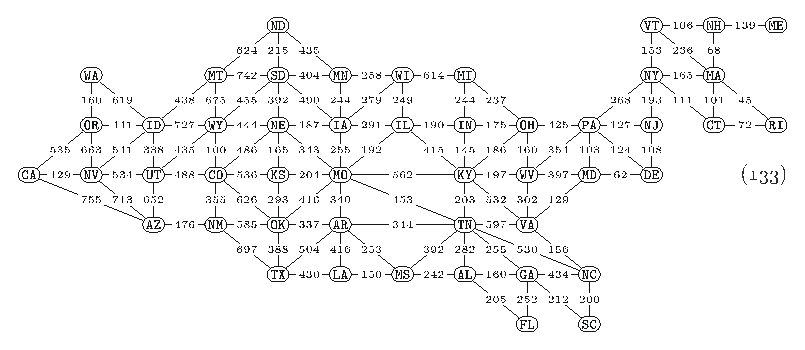
\includegraphics[width=0.9\linewidth]{fig/taocp_vol4fasc1b_p52_eq133.pdf}
  \caption{D.~E.~Knuth の教科書にある最短ハミルトン路問題の例}
  \label{fig:USmap}
\end{figure}
%%%%%%%%%%%%%%%%%%%%%%%%%%%%%%%%%

グラフの全頂点を一度ずつ通る路は
\textbf{ハミルトン路(Hamiltonian Path)}と呼ばれ,
閉路は
\textbf{ハミルトン閉路(Hamiltonian Cycle)}と呼ばれる.
以下に,本論文で対象とする問題群について述べる.

\begin{itemize}
\item \textbf{ハミルトン閉路問題}は,与えられたグラフの全頂点をちょう
  ど一度ずつ通る閉路が存在するかどうかを判定する問題である.
\item \textbf{ハミルトン路問題}は,ハミルトン閉路問題から始点と終点が
  一致するという閉路の条件を取り除いたものである.
\item \textbf{最短ハミルトン閉路問題}は,グラフの辺に距離が付随してい
  るとき,最短距離のハミルトン閉路を求める問題である.
\item \textbf{コスト制約付きハミルトン閉路問題}は,
  ハミルトン閉路問題に,距離の総和が所与の閾値以下(または以上)であるこ
  とを制約条件として付加した問題である\cite{comp20:Minato}.
\end{itemize}

図~\ref{fig:USmap}に,D.~E~.Knuth の教科書
The Art of Computer Programming~\cite{Knuth:TAOCP:SAT}
に記載されている最短ハミルトン路問題の例を示す.
このグラフは,米国本土48州の隣接関係を表しており,
頂点数は48,辺の数は105である.
各辺に付与されている数字は,州都の間の距離(マイル)を表している.
WA から ME までのハミルトン路は6,876,928通りあり,
最短ハミルトン路は11698マイルである~\cite{comp20:Minato}.

コスト制約付きハミルトン路問題は,WA から ME までの距離の総和がある
閾値以下であるハミルトン路を求める問題と考えることができる.
例えば,コスト制約を最短距離の10\%増(12,868マイル)以内とした場合,
解の総数は 16180 個である.

%%% Local Variables:
%%% mode: latex
%%% TeX-master: "paper"
%%% End:
